\documentclass{beamer}

\usetheme{default}

\usepackage{times}

\setbeamertemplate{navigation symbols}{}
\setbeamertemplate{footline}{
	\vbox{
		\hfill
		\usebeamerfont{framenumber}\insertframenumber/\inserttotalframenumber
		\hspace{2ex}
	}
	\noindent
\includegraphics[width=\textwidth]{LatexTemplates/bar.pdf}
}

\newcommand{\topBar}{
	\setbeamertemplate{headline}{
		
\includegraphics[width=\textwidth]{LatexTemplates/top.pdf}
	}
	\setbeamertemplate{footline}{
	}
}

\newcommand{\sponsorBar}{
	\setbeamertemplate{footline}{
		
\includegraphics[width=\textwidth]{LatexTemplates/sponsors.pdf}
	}
}

\usepackage{xpatch}
\xpatchcmd{\itemize}
{\def\makelabel}
	{\ifnum\@itemdepth=1\relax
		\setlength\itemsep{2ex plus 3ex minus 2ex}% separation for first level
	\else
	\ifnum\@itemdepth=2\relax
		\setlength\itemsep{1ex plus 2ex minus 1ex}% separation for second level
	\else
	\ifnum\@itemdepth=3\relax
		\setlength\itemsep{0.5ex plus 1ex minus 0.5ex}% separation for third level
\fi\fi\fi\def\makelabel
}{}{}



\usepackage{graphicx,xspace}
\usepackage{grffile}
\usepackage{hyperref}
\usepackage{url}

\begin{document}

%% Fill in here
\title{ICI3D LaTeX example}
\subtitle{Subtitle is optional} %% Comment out to omit
\author{Jonathan Dushoff}
\date{ICI3D 2017} %% For a talk, use event name, e.g. MMED 2017
\newcommand{\years}{2017} %% For copyright, typically the years talk has been givem
\newcommand{\figshare}{https://figshare.com/articles/NAME/NUMBER}

{
	\logo{
\includegraphics[width=1.5in]{ICI3D_logo.png}}

	\makeatletter
	\setbeamertemplate{sidebar canvas right}{}
	\setbeamertemplate{sidebar right}{%
		\vspace*{\fill}
		\llap{\insertlogo\hskip0.1cm}%
	}

	\makeatother

	\maketitle
}


\begin{frame}

\frametitle{Goals}

\begin{itemize}

\item Make a template

\item Make a clear example

\end{itemize}

\end{frame}
\begin{frame}

\frametitle{How do we use statistics}

\begin{itemize}

	\item We use statistics to confirm effects, estimate parameters, and
		predict outcomes

	\item It usually rains when I'm in Cape Town, but mostly on Sunday

	\begin{itemize}

		\item \emph{Confirmation:} In Cape Town, it rains more on Sundays than
				other days

		\item \emph{Estimation:} In Cape Town, the \emph{odds} of rain on
				Sunday are 1.6--2.2 times higher than on other days

		\item \emph{Prediction:} I am confident that it will rain at least one
				Sunday the next time I go

	\end{itemize}

\end{itemize}

\end{frame}

\begin{frame}

\frametitle{Raining in Cape Town}

\begin{columns}[c] \column{0.54\textwidth} \small

\begin{itemize}

	\item How we interpret data like this necessarily depends on assumptions:

	\begin{itemize}

		\item Is it likely our observations occured by chance?

		\item Is it likely they \emph{didn't}?

	\end{itemize}

\end{itemize}

\column{0.4\textwidth}

\hfill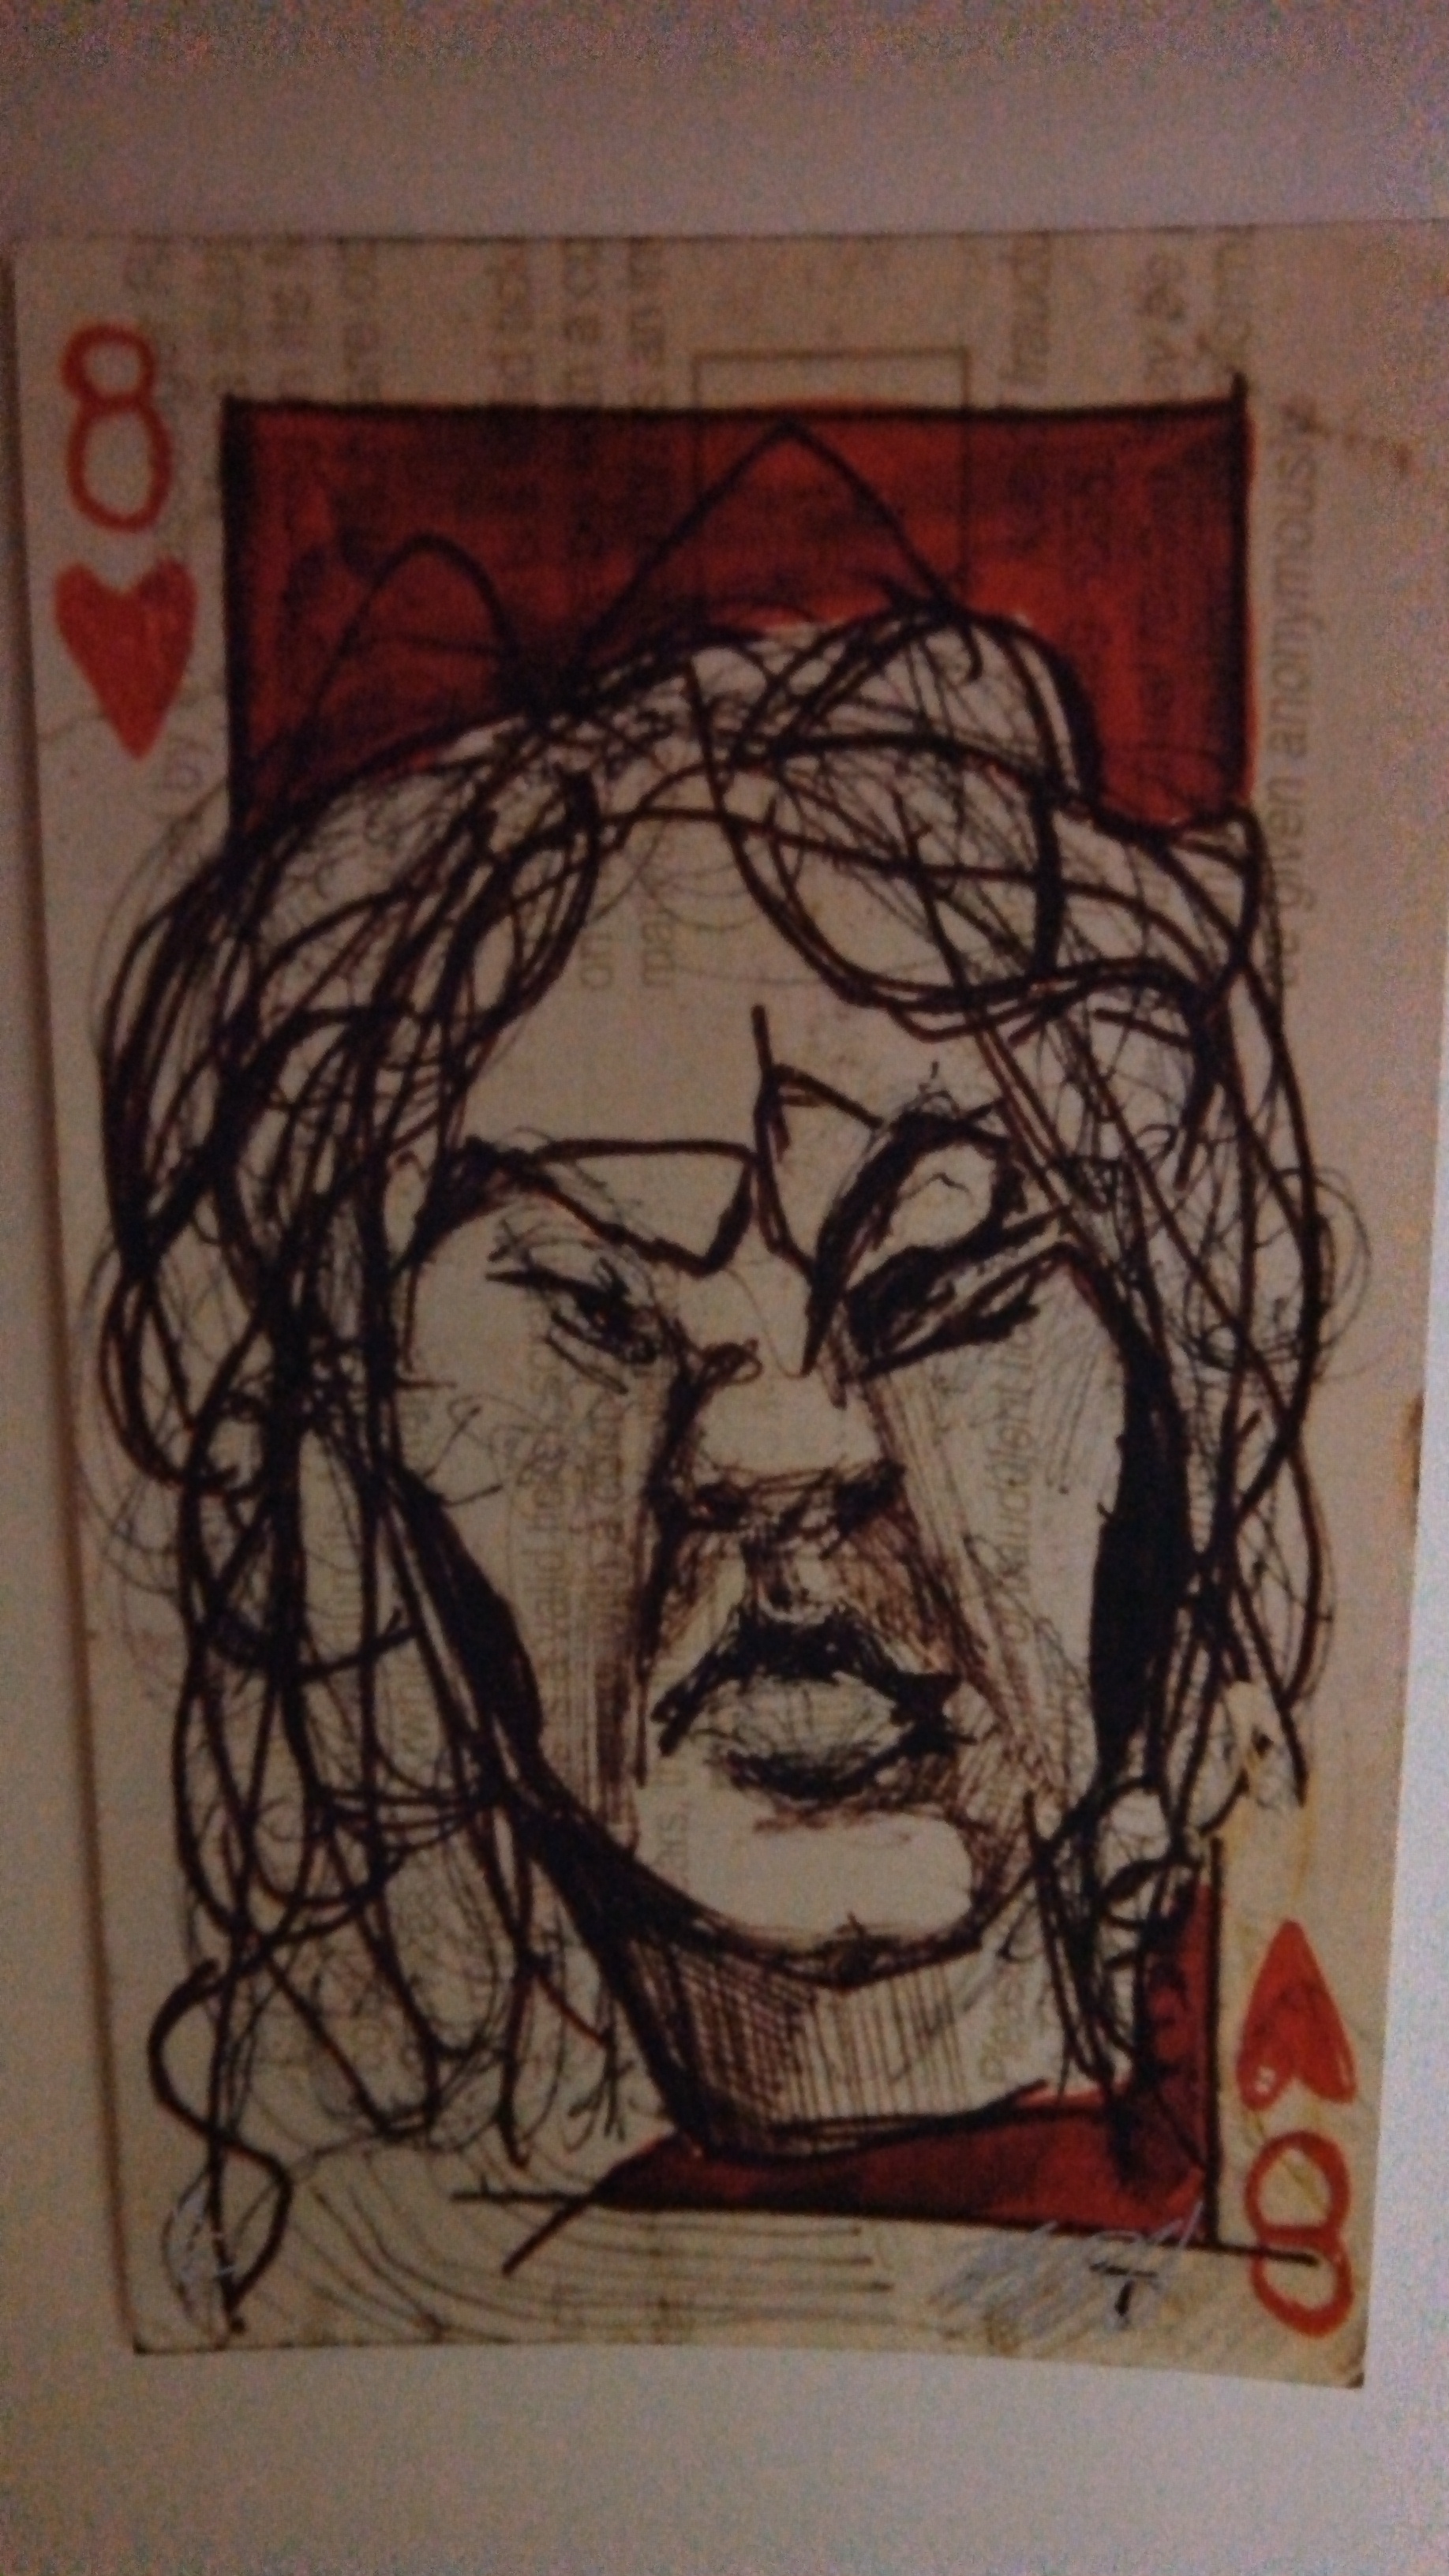
\includegraphics[height=0.8\textheight]{eight.jpg}\hfill\mbox{}

{\small\emph{Tessa Wessels, {\em Faces on a Train}}}

\end{columns}
\end{frame}

\begin{frame}

\frametitle{Goals}

\begin{itemize}

	\item We have made:

	\begin{itemize}

		\item a workable template

		\item a reasonably clear example (we hope)

	\end{itemize}

	\item Comments, questions, suggestions welcome

\end{itemize}

\end{frame}


\begin{frame}[plain]

\begin{centering}


\includegraphics[height=6ex]{rights.png}

\vfill

{
	\tiny\linespread{12}
	This presentation is made available through a Creative Commons Attribution-Noncommercial license.
	Details of the license and permitted uses are available at \url{http://creativecommons.org/licenses/by-nc/3.0/} \par
}

\medskip

\includegraphics[height=3ex]{attrib.png}
\hspace{3em}

\includegraphics[height=3ex]{noncom.png}
\medskip

{\tiny\copyright\years\ International Clinics on Infectious Disease Dynamics and Data}

\vfill

Title: {LECTURE TITLE}
Attribution: {LECTURER NAME}, Clinic on the Meaningful Modeling of Epidemiological Data
Source URL: {FIGSHARE URL}
For further information please contact \url{admin@ici3d.org}.

\vfill


\includegraphics[height=3ex]{AIMS.jpg}

\includegraphics[height=3ex]{sacema.png}

\includegraphics[height=3ex]{ICI3D_logo.png}

\end{centering}

\end{frame}


\end{document}
